\section{Application}

\begin{frame}{Application}
\begin{block}{}
    Encrypt message in QR codes using RECTANGLE
    \begin{itemize}
        \item encryptor.py - contains the encryption of RECTANGLE cipher 
        \item decryptor.py - contains the decryption of RECTANGLE cipher
        \item generate\_qr.py - encrypts the message and embeds it in QR code
        \item decrypt\_qr.py - scans and retrieves the plaintext from the QR-code
    \end{itemize}
        
\end{block}
\end{frame}

\begin{frame}{Generated QR Code}
\begin{block}{}
    \begin{figure}[h!]
    \centering
    % First Image
    \begin{subfigure}[b]{0.45\textwidth}
        \centering
        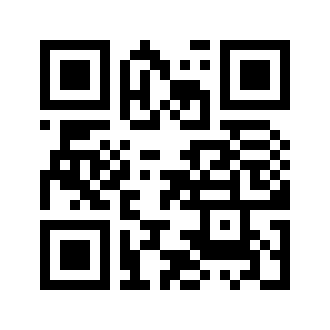
\includegraphics[width=\textwidth]{message.png} % Replace 'image1.png' with your image filename
        \label{fig:image1}
    \end{subfigure}
    \hfill
    % Second Image
    \begin{subfigure}[b]{0.45\textwidth}
        \centering
        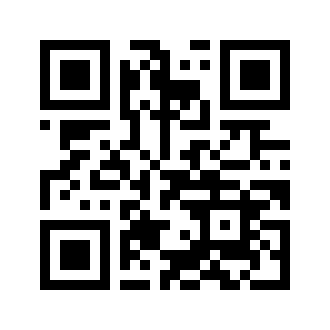
\includegraphics[width=\textwidth]{birth.png} % Replace 'image2.png' with your image filename
        \label{fig:image2}
    \end{subfigure}

    \caption{Above QR Codes contain encrypted messages}
    \label{fig:two_images}
\end{figure}
        
\end{block}
\end{frame}